
\section{Solving a Real Use Case: Function Visualization}

In this section, we assume that you want to visualize two functions. The first
function is given by means of a data table. The second function is given by
means of a math expression. We would like to place the two results side by
side, and we would like to have ``proper'' alignment (whatever that means).

As motivated, we have one data table. Let us assume that it is as shown below.
%
\begin{codeexample}[code only]
x_0	f(x)
# some comment line
3.16693000e-05	-4.00001451e+00
1.00816962e-03	-3.08781504e+00
1.98466995e-03	-2.88058811e+00
2.96117027e-03	-2.75205040e+00
3.93767059e-03	-2.65736805e+00
4.91417091e-03	-2.58181091e+00
5.89067124e-03	-2.51862689e+00
...
9.89226496e-01	2.29825980e+00
9.90202997e-01	2.33403276e+00
9.91179497e-01	2.37306821e+00
9.92155997e-01	2.41609413e+00
9.93132498e-01	2.46412019e+00
9.94108998e-01	2.51860712e+00
9.95085498e-01	2.58178769e+00
9.96061999e-01	2.65733975e+00
9.97038499e-01	2.75201383e+00
9.98014999e-01	2.88053559e+00
9.98991500e-01	3.08771757e+00
9.99968000e-01	3.99755546e+00
\end{codeexample}
%
Note that parts of the data file have been omitted here because it is a bit
lengthy. The data file (and all others referenced in this manual) are shipped
with \PGFPlots{}; you can find them in the subfolder
\texttt{doc/latex/pgfplots/plotdata}.


\subsection{Getting the Data Into \TeX{}}
\label{sec:tut1:step1}

Our first step is to get the data table into \PGFPlots{}. In addition, we want
axis descriptions for the |x| and |y| axes and a |title| on top of the plot.

Our first version looks like
%
\begin{codeexample}[]
%\documentclass{article}
%\usepackage{pgfplots}
%\pgfplotsset{compat=1.5}

%\begin{document}

\begin{tikzpicture}
\begin{axis}[
    title=Inv. cum. normal,
    xlabel={$x$},
    ylabel={$y$},
]
    \addplot [blue] table {invcum.dat};
\end{axis}
\end{tikzpicture}
%\end{document}
\end{codeexample}

The code listing already shows a couple of important aspects:
%
\begin{enumerate}
    \item As usual in \LaTeX{}, you include the package using
        |\usepackage{pgfplots}|.
    \item Not so common is |\pgfplotsset{compat=1.5}| .

        A statement like this should always be used in order to (a)~benefit
        from a more or less recent feature set and (b)~avoid changes to your
        picture if you recompile it with a later version of \PGFPlots{}.

        Note that \PGFPlots{} will generate some suggested value into your
        logfile (since 1.6.1). The minimum suggested version is
        |\pgfplotsset{compat=1.3}| as this has great effect on the
        positioning of axis labels.
    \item \PGFPlots{} relies on \Tikz{} and \pgfname{}. You can say it is a
        ``third party package'' on top of \Tikz{}/\pgfname{}.

        Consequently, we have to write each \PGFPlots{} graph into a \Tikz{}
        picture, hence the picture environment given by
        |\begin{tikzpicture} ... \end{tikzpicture}|.
    \item Each axis in \PGFPlots{} is written into a separate environment. In
        our case, we chose |\begin{axis} ... \end{axis}| as this is the
        environment for a normal axis.

        There are more axis environments (like the
        |\begin{loglogaxis} ... \end{loglogaxis}| environment for logarithmic
        axes).

        Although \PGFPlots{} runs with default options, it accepts keys. Lots
        of keys. Typically, you provide all keys which you ``want to have''
        in square brackets ``somewhere'' and ignore all other keys.

        Of course, the main difficulty is to get an overview over the available
        keys and to find out how to use them. This reference manual and
        especially its Chapter~\ref{cha:pgfplots:reference} has been designed
        for online browsing: it contains hundreds of cross-referenced examples.
        Opening the manual in a PDF viewer and searching it for keywords will
        hopefully jump to a good match from which you can jump to \emph{the}
        reference section (for example about tick labels, tick positions, plot
        handlers, etc.). It is (and will always be) the most reliable source of
        detail information about all keys.

        Speaking about the reference manual: note that most PDF viewers also
        have a function to ``jump back to the page before you clicked on a
        hyperlink'' (for Acrobat Reader, open the menu View / Toolbars / More
        Tools and activate the ``Previous View'' and ``Next View'' buttons
        which are under ``Page Navigation Toolbar'').

        Note that the code listing contains two sets of keys: the first is
        after |\begin{axis}[ ... ]| and the second right after
        |\addplot[...]|. Note furthermore that the option list after the axis
        has been indented: each option is on a separate line, and each line
        has a tab stop as first character. This is a good practice. Another
        good practice is to place a comma after the last option (in our case,
        after the value for |ylabel|). This allows to add more keys easily --
        and you won't forget the comma. It does not hurt at all. The second
        ``set'' of keys after |\addplot| shows that indentation and trailing
        comma a really just a best practice: we simply said |\addplot[blue]|,
        meaning that the plot will be placed in blue color, without any plot
        |mark|. Of course, once another option would be added here, it would
        be best to switch to indentation and trailing comma:
        %
\begin{codeexample}[code only]
\addplot[
    blue,
    mark=*,
]
table {invcum.dat};
\end{codeexample}
        %
    \item Inside of an axis, \PGFPlots{} accepts an |\addplot ... ;|
        statement (note the final semicolon).

        In our case, we use |\addplot table|: it loads a table from a file
        and plots the first two columns.

        There are, however, more input methods. The most important available
        inputs methods are |\addplot expression| (which samples from some
        mathematical expression) and |\addplot table| (loads data from
        tables), and a combination of both which is also supported by
        |\addplot table| (loads data from tables and applies mathematical
        expressions). Besides those tools which rely only on built-in
        methods, there is also an option to calculated data using external
        tools: |\addplot gnuplot| which uses gnuplot as ``desktop
        calculator'' and imports numerical data, |\addplot shell| (which can
        load table data from any system call), and the special
        |\addplot graphics| tool which loads an \emph{image} together with
        meta data and draws only the associated axis.

        In our axis, we find a couple of tokens: the first is the mandatory
        |\addplot| token. It ``starts'' a further plot. The second is the
        option list for that plot, which is delimited by square brackets (see
        also the notes about best practices above). The name ``option list''
        indicates that this list can be empty. It can also be omitted
        completely in which case \PGFPlots{} will choose an option list from
        its current |cycle list| (more about that in a different lecture).
        The next token is the keyword ``|table|''. It tells \PGFPlots{} that
        table data follows. The keyword ``|table|'' also accepts an option
        list (for example, to choose columns, to define a different |col sep|
        or |row sep| or to provide some math expression which is applied to
        each row). More on that in a different lecture. The next token is
        |{invcum.dat}|: an argument in curly braces which provides the table
        data. This argument is interpreted by ``plot table''. Other input
        types would expect different types of arguments. In our case, the
        curly braces contain a file name. Plot table expects either a file
        name as in our case or a so-called ``inline table''. An inline table
        means that you would simply insert the contents of your file inside
        of the curly braces. In our case, the table is too long to be
        inserted into the argument, so we place it into a separate file.
        Finally, the last (mandatory!) token is a semicolon. It terminates
        the |\addplot| statement.
    \item Axis descriptions can be added using the keys
        |title, xlabel, ylabel| as we have in our example listing.

        \PGFPlots{} accepts lots of keys -- and sometimes it is the art of
        finding just the one that you were looking for. Hopefully, a search
        through the table of contents of the reference manual and/or a
        keyword search through the entire reference manual will show a hit.
\end{enumerate}


\subsection{Fine-Tuning of the First Picture}
\label{sec:tut1:step2}

While looking at the result of Section~\ref{sec:tut1:step1}, we decide that we
want to change something. First, we decide that the open ends on the left and
on the right are disturbing (perhaps we have a strange taste -- or perhaps we
know in advance that the underlying function is not limited to any interval).
Anyway, we would like to show it only in the |y| interval from $-3$ to $+3$.

We can do so as follows:
%
\begin{codeexample}[]
\begin{tikzpicture}
\begin{axis}[
    title=Inv. cum. normal,
    xlabel={$x$},
    ylabel={$y$},
    ymin=-3, ymax=3,
    minor y tick num=1,
]
    \addplot [blue] table {invcum.dat};
\end{axis}
\end{tikzpicture}
\end{codeexample}

We added three more options to the option list of the axis. The first pair is
|ymin=-3| and |ymax=3|. Note that we have placed them on the same line although
we said the each should be on a separate line. Line breaks are really optional;
and in this case, the two options appear to belong together. They define the
\emph{display} limits. Display limits define the ``window'' of the axis. Note
that any |\addplot| statements might have more data (as in our case). They
would still generate graphics for their complete set of data points! The keys
|ymin,ymax,xmin,xmax| control only the \emph{visible} part, i.e.\@ the axis
range. Everything else is clipped away (by default). The third new option is
|minor y tick num=1| which allows to customize minor ticks. Note that minor
ticks are only displayed if the major ticks have the same distance as in our
example.

Note that we could also have modified the |width| and/or |height| of the figure
(the keys have these names). We could also have used one of the predefined
styles like |tiny| or |small| in order to modify not just the graphics, but
also use different fonts for the descriptions. We could also have chosen to
adjust the unspecified limits: either by fixing them explicitly (as we did for
y above) or by modifying the |enlargelimits| key (for example using
|enlargelimits=false|).

We are now satisfied with the first picture and we would like to add the second
one.


\subsection{Adding the Second Picture with a Different Plot}
\label{sec:tut1:step3}

As motivated, our goal is to have two separate axes placed side by side. The
second axis should show a function given as math expression. More precisely, we
want to show the density function of a normal distribution here (which is just
a special math expression).

We simply start a new |tikzpicture| and insert a new |axis| environment
(perhaps by copy--pasting our existing one). The |\addplot| command is
different, though:

\begin{codeexample}[]
\begin{tikzpicture}
\begin{axis}[
]
    % density of Normal distribution:
    \addplot [
        red,
        domain=-3e-3:3e-3,
        samples=201,
    ]
        {exp(-x^2 / (2e-3^2)) / (1e-3 * sqrt(2*pi))};
\end{axis}
\end{tikzpicture}
\end{codeexample}

We see that it has an axis environment with an empty option list. This is quite
acceptable: after all, it is to be expected that we will add options
eventually. Even if we don't: it does not hurt. Then, we find the expected
|\addplot| statement. As already explained, |\addplot| statements initiate a
new plot. It is followed by an (optional) option list, then by some keyword
which identifies the way input coordinates are provided, then arguments, and
finally a semicolon. In our case, we find an option list which results in a red
plot. The two keys |domain| and |samples| control how our math expression is to
be evaluated: |domain| defines the sampling interval in the form |a:b| and
|samples=N| expects the number of samples inserted into the sampling interval.
Note that |domain| merely controls which samples are taken; it is independent
of the displayed axis range (and both can differ significantly). If the keyword
defining how coordinates are provided is missing, \PGFPlots{} assumes that the
next argument is a math expression. Consequently, the first token after the
option list is a math expression in curly braces. We entered the density
function of a normal distribution here (compare
\href{http://en.wikipedia.org/wiki/Normal_distribution}{Wikipedia}).

Note that the axis has an axis multiplier: the $x$ tick labels have been chosen
to be $-2$, $0$, and $2$ and an extra $x$ tick scale label of the form `$\cdot
10^{-3}$'. These tick scale labels are quite convenient are are automatically
deduced from the input data. We will see an example with the effects of
|scaled x ticks=false| at the end of this tutorial.

Inside of the math expression, you can use a lot of math functions like exp,
sin, cos, sqrt, you can use exponents using the |a^b| syntax, and the sampling
variable is |x| by default. Note, however, that \emph{trigonometric functions
operate on degrees} by default! If you need to sample the sinus function, you
can use |\addplot[domain=0:360] {sin(x)};|. This is quite uncommon. You can
also use |\addplot[domain=0:2*pi] {sin(deg(x)};|. This samples radians (which
is more common). But since the math parser expects degrees, we have to convert
|x| to degrees first using the |deg()| function. See also
|trig format plots=rad|. The math parser is written in \TeX{} (it does not need
any third-party tool). It supports the full range of a double precision number,
even though the accuracy is about that of a single precision number. This is
typically more than sufficient to sample any function accurately. If you ever
encounter difficulties with precision, you can still resort to
|\addplot gnuplot| in order to invoke the external tool gnuplot as ``coordinate
calculator''.

The experienced reader might wonder about \emph{constant} math expressions
|domain=-3e-3:3e-3|, |2e-3^2|, and |1e-3| rather than some variable name like
`|mu|' or `|sigma|'. This is actually a
matter of taste: both is supported and we will switch to variable names in the
next listing.

The main part of our step here is still to be done: we wanted to place two
figures side by side. This can be done as follows:
%
\begin{codeexample}[]
\begin{tikzpicture}
    \begin{axis}[
        title=Inv. cum. normal,
        xlabel={$x$},
        ylabel={$y$},
        ymin=-3, ymax=3,
        minor y tick num=1,
    ]
        \addplot [blue] table {invcum.dat};
    \end{axis}
\end{tikzpicture}% -- avoid white space
%
\hskip 10pt % insert a non-breaking space of specified width.
%
\begin{tikzpicture}
    \begin{axis}[
    ]
        % density of Normal distribution:
        \newcommand\MU{0}
        \newcommand\SIGMA{1e-3}
        \addplot[
           red,
           domain=-3*\SIGMA:3*\SIGMA,
           samples=201,
        ]
           {exp(-(x-\MU)^2 / 2 / \SIGMA^2) / (\SIGMA * sqrt(2*pi))};
    \end{axis}
\end{tikzpicture}
\end{codeexample}

The listing above shows the two separate picture environments: the first is
simply taken as is from the previous step and the second is new. Note that both
are simply placed adjacent to each other: we only inserted comment signs to
separate them. This approach to place graphics side by side is common in
\TeX{}: it works for |\includegraphics| in the same way. You could, for
example, write
%
\begin{codeexample}[code only]
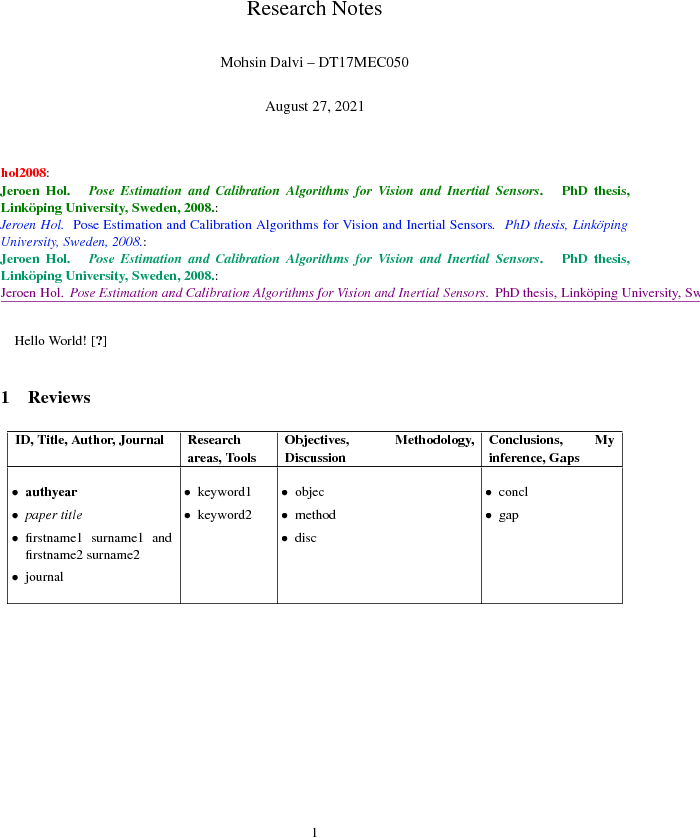
\includegraphics{image1}%
%
\hskip 10pt % insert a non-breaking space of specified width.
%
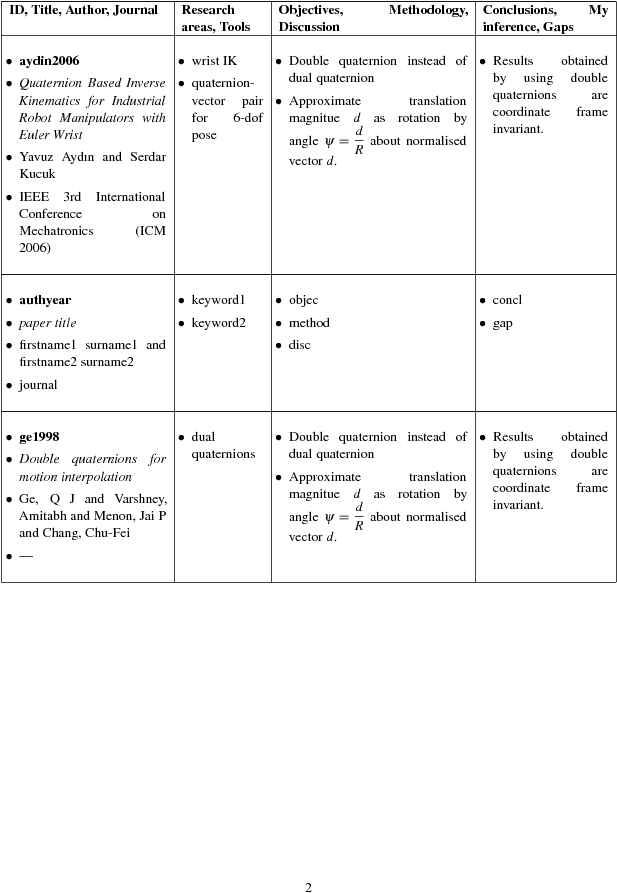
\includegraphics{image2}
\end{codeexample}
%
to place two graphics next to each other. This here is just the same (except
that our graphics occupy more code in the |.tex| file).

Note that there is also a comment sign after |\end{tikzpicture}|. This is not
just a best practice: it is necessary to suppress spurious spaces! In \TeX{},
every newline character is automatically converted to a white space (unless you
have an empty line, of course). In our case, we want no white spaces.

In our second picture, we see the effects of switch our math expression to
constant definitions as promised earlier. The interesting part starts with two
constants which are defined by means of two |\newcommand|s: we define |\MU| to
be 0 and |\SIGMA| to be |1e-3|. This is one way to define constants (note that
such a definition of constants should probably introduce round braces if
numbers are negative, i.e.\@ something like |\newcommand\negative{(-4)}|).


\subsection{Fixing the Vertical Alignment and Adjusting Tick Label Positions}
\label{sec:tut1:step4}

Note that even though our individual pictures look quite good, the combination
of both is not properly aligned. The experienced reader identifies the weak
point immediately: the bounding box of the two images differs, and they are
aligned at their baseline (which is the bottom edge of the picture). In
particular, the |xlabel=$x$| of the left picture and the automatically inserted
scaling label |\cdot 10^{-3}| of the right picture cause an unwanted vertical
shift. We want to fix that in the next step.

Besides the bad alignment, we find it a little bit misleading that the axis
descriptions of the second picture are between both pictures. We would like to
move them to the right.

Let us present the result first:
%
\begin{codeexample}[]
\begin{tikzpicture}[baseline]
    \begin{axis}[
        title=Inv. cum. normal,
        xlabel={$x$},
        ylabel={$y$},
        ymin=-3, ymax=3,
        minor y tick num=1,
    ]
        \addplot [blue] table {invcum.dat};
    \end{axis}
\end{tikzpicture}%
%
\hskip 10pt % insert a non-breaking space of specified width.
%
\begin{tikzpicture}[baseline]
    \begin{axis}[
        yticklabel pos=upper,
    ]
        % density of Normal distribution:
            \newcommand\MU{0}
            \newcommand\SIGMA{1e-3}
        \addplot [red,domain=-3*\SIGMA:3*\SIGMA,samples=201]
            {exp(-(x-\MU)^2 / 2 / \SIGMA^2) / (\SIGMA * sqrt(2*pi))};
    \end{axis}
\end{tikzpicture}
\end{codeexample}
%
This listing has a couple of modifications. The most important one is the we
added an option list to the |tikzpicture| environment: the |baseline| option.
This option shifts the picture up or down such that the canvas coordinate $y=0$
is aligned at the baseline of the surrounding text. In \PGFPlots{}, the $y=0$
line is the lower edge of the box. This simple feature allows both axes to be
aligned vertically: now, their boxes are aligned rather than the lower edges of
their bounding boxes. The option baseline needs to be provided to all pictures
for which this shifting should be done -- in our case, to all which are to be
placed in one row. Keep in mind that it is an option for |\begin{tikzpicture}|.

The second change is rather simple: we only added the option
|yticklabel pos=upper| to the second axis. This moves all tick labels to the
right, without changing anything else.

Note that there is much more to say about alignment and bounding box control.
After all, we did not really change the bounding box -- we simply moved the
pictures up or down. There is also the use case where we want horizontal
alignment: for example if the two pictures should be centered horizontally or
if they should be aligned with the left- and right end of the margins. The
associated keys |\begin{tikzpicture}[trim axis left, trim axis right]| and
|\centering| are beyond the scope of this tutorial, please refer to
Section~\ref{pgfplots:sec:align} for details.


\subsection{Satisfying Different Tastes}
\label{sec:tut1:step5}

We are now in a position where the figures as such are in a good shape.

However, an increase in knowledge will naturally lead to an increase in
questions. Some of these questions will be part of other how-to lectures. But
the most commonly asked questions are addressed here (feel free to email some
more if you believe that I should include another hotspot):
%
\begin{enumerate}
    \item How can I get rid of that $10^{-3}$ label?
    \item How can I modify the number printing?
    \item How can I have one single line per axis rather than a box?
\end{enumerate}

This here gives brief hints where to look in this reference manual for more
details. We modify the appearance of the second picture according to the
questions above:
%
\begin{codeexample}[]
\begin{tikzpicture}
\begin{axis}[
    axis lines=left,
    scaled ticks=false,
    xticklabel style={
        rotate=90,
        anchor=east,
        /pgf/number format/precision=3,
        /pgf/number format/fixed,
        /pgf/number format/fixed zerofill,
    },
]
    % density of Normal distribution:
        \newcommand\MU{0}
        \newcommand\SIGMA{1e-3}
  \addplot [red,domain=-3*\SIGMA:3*\SIGMA,samples=201]
        {exp(-(x-\MU)^2 / 2 / \SIGMA^2)
            / (\SIGMA * sqrt(2*pi))};
\end{axis}
\end{tikzpicture}
\end{codeexample}

The appearance of the axes as such can be controlled by means of the
|axis lines| key. It accepts the values |left, right, box, center, none| (and
also |top, bottom, middle| which are aliases). The |xticklabel style| key
modifies a predefined style (note the use of indentation here!). A style is a
collection of keys which are applied in a specific context. Styles are very
useful and are widely used by \PGFPlots{}. In our case, we adjust a couple of
options like rotation, alignment (the |anchor| option), and number printing
options. The precise details of these individual options is beyond the scope of
this tutorial. The keys actually belong to \Tikz{} -- and the \Tikz{} manual is
the reference for these keys (although \PGFPlots{} also covers most of the
topics). The complete set of number printing options is available in both the
\Tikz{} manual~\cite{tikz} and the manual for \PGFPlotstable{} which is shipped
with \PGFPlots{}. A brief extract can be found in
Section~\ref{sec:number:printing}.


\subsection{Finishing Touches: Automatic Generation of Individual Pdf Graphics}
\label{sec:tut1:step6}

As last step in this lecture, I would like to talk about one technical topic.
Typically, a \TeX{} document starts quite simple: a little bit of text, perhaps
one or two pictures. But they tend to grow. And eventually, you will encounter
one of the weak points of \PGFPlots{}: the graphics are involved and \TeX{}
consumes a lot of time to generate them. Especially if it keeps regenerating
them even though they did not change at all. The fact that we need to rerun the
pdflatex processor all the time makes things worse.

Fortunately, there are solutions. A simple solution is: why can't we write each
individual graphics into a separate |.pdf| file and use |\includegraphics| to
include it!? The answer is: yes, we can. And it is surprisingly simple to do
so.

In order to convert every |tikzpicture| environment automatically to an
external graphics \emph{without} changing any line of code in the \TeX{} file,
we can simply write the following two lines into the document's preamble:
%
\begin{codeexample}[code only]
\usepgfplotslibrary{external}
\tikzexternalize

...
\begin{document}
...
\end{document}
\end{codeexample}
%
But now, we \emph{have to provide a command line switch to pdflatex}:
%
\begin{codeexample}[code only]
pdflatex -shell-escape myfile.tex
\end{codeexample}

This works out of the box with |pdflatex|. If you use |latex/dvips|,
|lualatex|, |dvipdfm| or any other \TeX{} derivatives, you need to modify the
option |\tikzexternalize[system call=...]| (which is, unfortunately,
system-dependent, especially for the postscript variants).

It might be too much to discuss how to define individual file names or how to
modify the file name generation strategy. There is also the
|\tikzexternalize[mode=list and make]| feature which generates a GNU Make file
to allow |\label/\ref| to things inside of the external graphics and which
supports the generation of all images in parallel (if you have a multi-core
PC).

Details of the |external| library can be found in
Section~\ref{sec:pgfplots:export} (but only a brief survey) and, in all depth,
in the \Tikz{} reference manual~\cite{tikz}.


\subsection{Summary}

We learned how to create a standard axis, and how to assign basic axis
descriptions. We also saw how to plot functions from a data table (in our case
a tab-separated file, but other delimiters as in CSV files are also supported)
and from math expressions. We saw that \PGFPlots{} does a reasonable good job
at creating a fully-featured axis automatically (like scaling the units
properly, choosing tick positions and labels). We also learned how to improve
vertical alignment and how to customize the appearance of an axis.

Next steps might be how to draw multiple plots into the same axis, how to
employ scatter plots of \PGFPlots{}, how to generate logarithmic axes, or how
to draw functions of two variables. Some of these aspects will be part of
further how-to lectures.
